\chapter{The Large Hadron Collider and the CMS Experiment}
\label{chap:hardware}

In order to study the properties of the Standard Model particles, and
to search for physics beyond the Standard Model, we need a way to
produce particles other than the simple up and down quarks and
electrons that make up everyday matter. And once we have produced such
particles, we need a way to detect their presence, identify them, and
measure their properties.

This chapter will describe the machines used to perform
the analyses described in Chapters \ref{chap:afb} and \ref{chap:stop},
namely the Large Hadron Collider and the CMS Detector. It
will also describe how the CMS Collaboration uses software to make sense of
the readings it has collected from the CMS detector. Because these
systems are immensely complex, this chapter will not attempt to
describe these systems in exhaustive detail, but will focus on the details that are
important for understanding the science presented in the next two
chapters. % Review to see if I'm actually meeting this goal

\section{The Large Hadron Collider}
\label{sec:lhc}

In order to study heavy particles, we must first create them, since
it is impractical to find them in nature.
Einstein's famous equation, $E = mc^2$, tells us that mass and energy
are equivalent to one another. Physicists employ this principle to create
heavier particles by taking lightweight particles, accelerating them to very high
speeds, and smashing them together. Particles moving at high speed
have high kinetic energy, and when those particle collide, that energy
can be converted into mass, creating heavier particles. Because it is
so often conducted at high energies, particle physics is sometimes
referred to as high energy physics, or HEP.

The Large Hadron Collider, or LHC, is the largest and most
powerful particle collider ever built.
It is the flagship project of CERN, the European Organization
for Nuclear Research, located in Geneva, Switzerland.
The LHC is a ring-shaped structure about 27 kilometers (17 miles) in circumference,
buried underground beneath the border between Switzerland and
France, as shown in Figure \ref{fig:lhc:above}. The ring encloses two
pipes, through which beams of protons normally circulate in opposite
directions for eventual collision. Strong electric fields propel the protons along the beam
pipes, and strong magnetic fields steer the protons around the ring
\cite{lhc}. The LHC tunnel and a cutaway view inside the accelerator
may be seen in Figure \ref{fig:lhc:cutaway}.

% Picture of the LHC from above
\begin{figure}[htb]
\centering
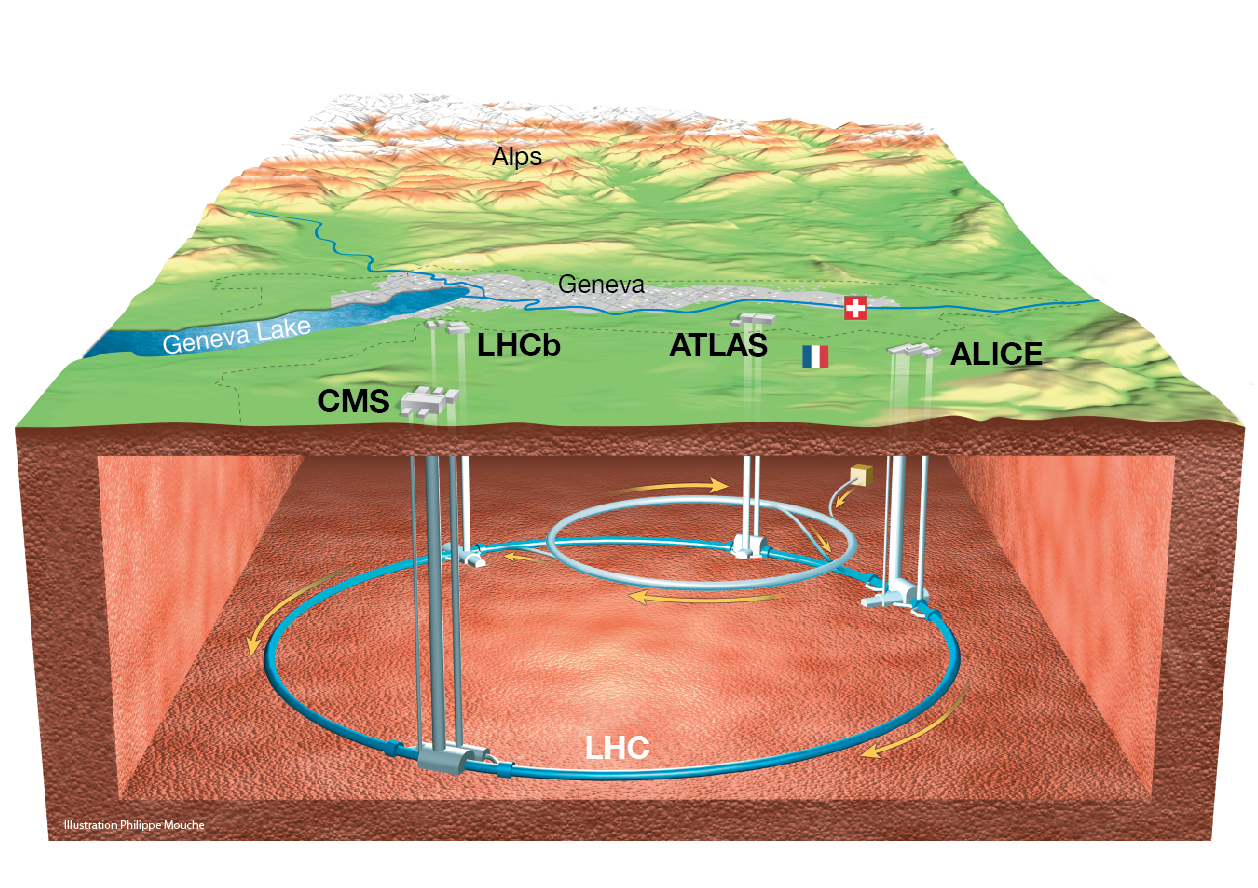
\includegraphics[width=0.9\textwidth]{figures/lhc-from-above.png}
\caption[Situation of the Large Hadron Collider near Geneva,
Switzerland.]{Situation of the Large Hadron Collider near Geneva,
  Switzerland \cite{cernphotos}.}
\label{fig:lhc:above}
\end{figure}

% Picture of the LHC tunnel, with cutaway view of the cryomodules
\begin{figure}[htb]
\centering
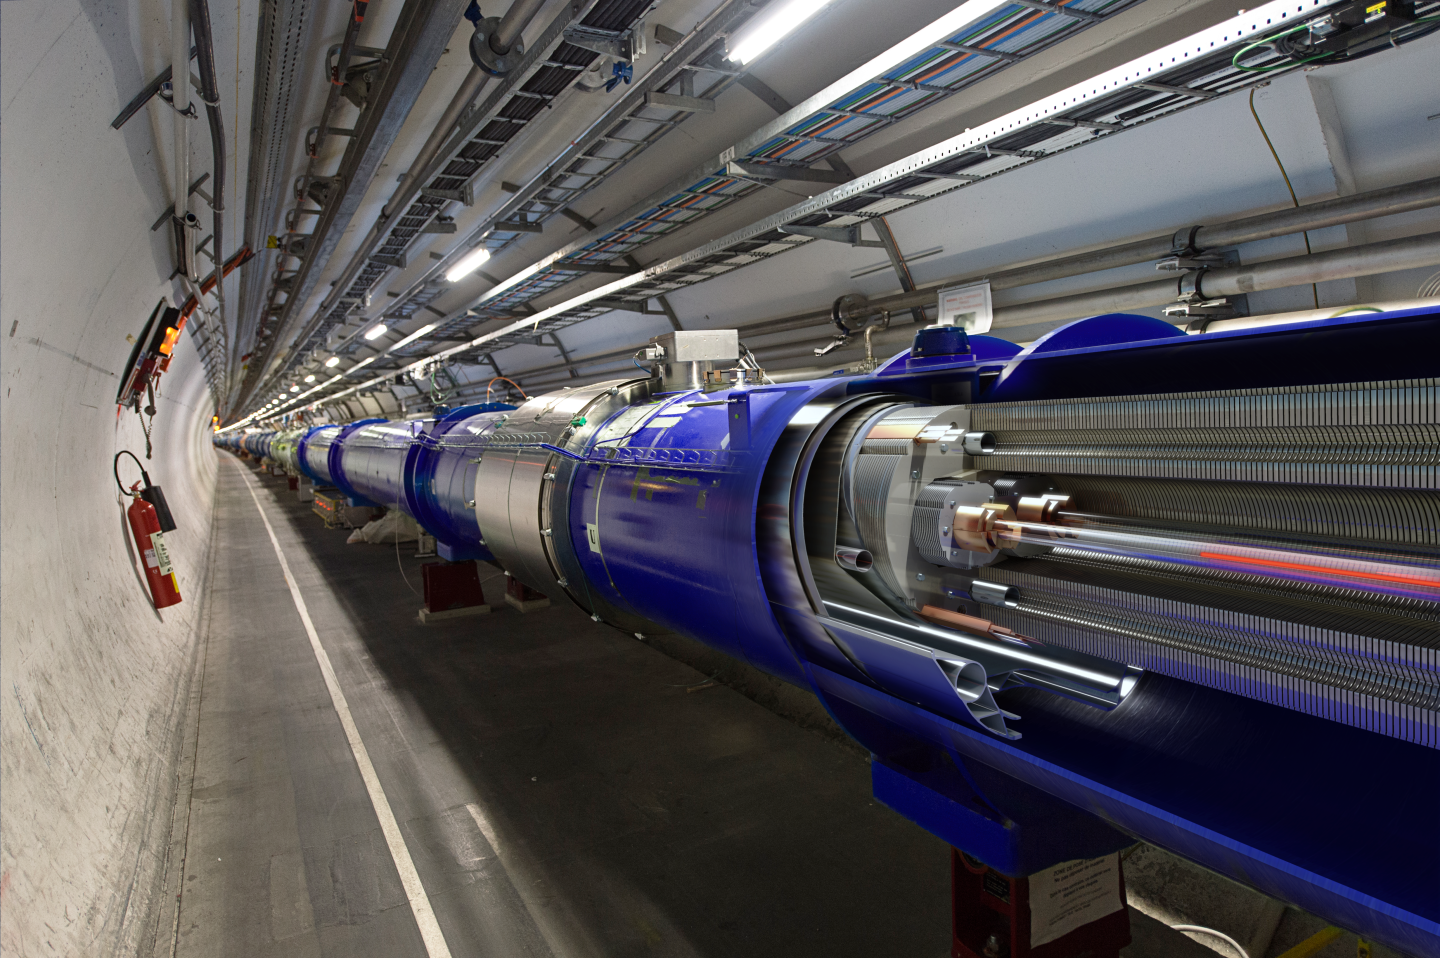
\includegraphics[width=0.9\textwidth]{figures/lhc-tunnel-cutaway.png}
\caption[Interior of the LHC tunnel, with cutaway view inside the
  accelerator.]{Interior of the LHC tunnel, with cutaway view inside
    the accelerator \cite{cernphotos}.}
\label{fig:lhc:cutaway}
\end{figure}

The LHC is fed by a chain of smaller accelerators at CERN that shape
the beams and bring them partway up to speed so they can be injected
into the LHC. The LHC was designed to collide protons at an energy of
14 trillion electron volts (TeV). However, during early testing, a
defective weld caused severe damage to the LHC; as a precaution
against future damage, the LHC was operated at 7 and 8 TeV energy in
its first run (Run I), and has been colliding at 13 TeV so far in its
second run (Run II). At these energies, the protons in the beam are
moving at 99.999999\% of the speed of light.

The proton beams are not continuous streams of particles. Rather, the
protons are grouped into bunches. The LHC is designed to circulate
2808 bunches of protons in each direction, with each bunch containing
about 120 billion protons when it is first injected.
The total ``amount of beam'' delivered per unit time is called
\emph{luminosity}, denoted $\mathcal{L}$. Unrelated to the measure of
optical power, luminosity in accelerator physics is expressed in
units of 1/(area$\times$time); the typical luminosity of the LHC integrated over one
year of running is on the order of several dozen
\emph{inverse femtobarns} (fb\textsuperscript{-1}). The strange
choice of units for luminosity allows us to express it as the inverse of
\emph{cross section} (denoted $\sigma$), which is measured in units
of area. The cross section for a particular process is a kind of
relative probability of that process occurring. Because time-integrated
luminosity has units of inverse area, the number of occurrences, $N$,
of a given process observed in some time is given by:
\begin{equation}
N = \mathcal{L}_\text{int} \cdot \sigma
\end{equation}
Thus a process with a cross section of 50 fb may be expected
to occur 1000 times in 20 fb\textsuperscript{-1} of data.

The proton beams are made to collide every 25ns, or 40 million times
per second. Each beam crossing is referred to as an ``event''. A
single event typically contains about 20 collisions between the
protons in the bunches, though only one collision in the event will be
analyzed. Usually this is the most energetic collision. The products
of any secondary collisions are known as \emph{pileup}, and are
treated as general background debris to be subtracted out.

Although we have been describing protons as simple particles, in fact
they are anything but. Protons contain two up quarks and a down quark,
and innumerable gluons binding them together. But in addition, protons
contain a sort of froth of quarks and antiquarks that are constantly
popping into and out of existence on ultrashort timescales, in
accordance with the laws of quantum mechanics. Collectively, all of
these components of a proton are known as \emph{partons}, and any of
them may be involved when two protons collide. Studies on the relative
momentum of the various partons tell us that at the LHC, most of the
time it is the gluons that are colliding with each other. % Citation?

At the LHC, there are four places where the beam pipes intersect and
the proton beams are made to collide with one another. At each of these
four locations, a detector is placed where it can observe the
particles that are produced by these collisions. Two of
the detectors are large, general-purpose machines, designed to support
a broad range of particle physics research. These detectors are called CMS
and ATLAS. There are two general-purpose detectors so that the results from one
may be cross-checked by the other. The other two main
detectors are moderately sized and designed to study specific kinds of physics
phenomena. One is LHCb, which is designed to study the physics of
bottom quarks. The other is ALICE; a few weeks each year, the LHC
collides lead nuclei instead of protons, and ALICE is designed to
study the physics of these collisions. In recent years, three smaller detectors have
been added: ToTeM, which shares an interaction point with CMS; MoEDAL,
which is colocated with LHCb; and LHCf, installed around the ATLAS detector.

\section{The CMS Detector}
\label{sec:cms}

The research described in Chapters \ref{chap:afb} and \ref{chap:stop}
was conducted using data gathered on proton-proton collisions by the
CMS detector. CMS stands for Compact Muon Solenoid, a name whose
origin will become apparent in the next few sections. In brief, though,
this detector is a complex, multilayered array of sensors designed to
detect and measure the properties of as many of the particles emerging
from the collision point as possible \cite{cms}. Figure
\ref{fig:cms:outside} provides a cutaway view inside these layers.

% Picture of the CMS detector with cutaway view
\begin{figure}[htb]
\centering
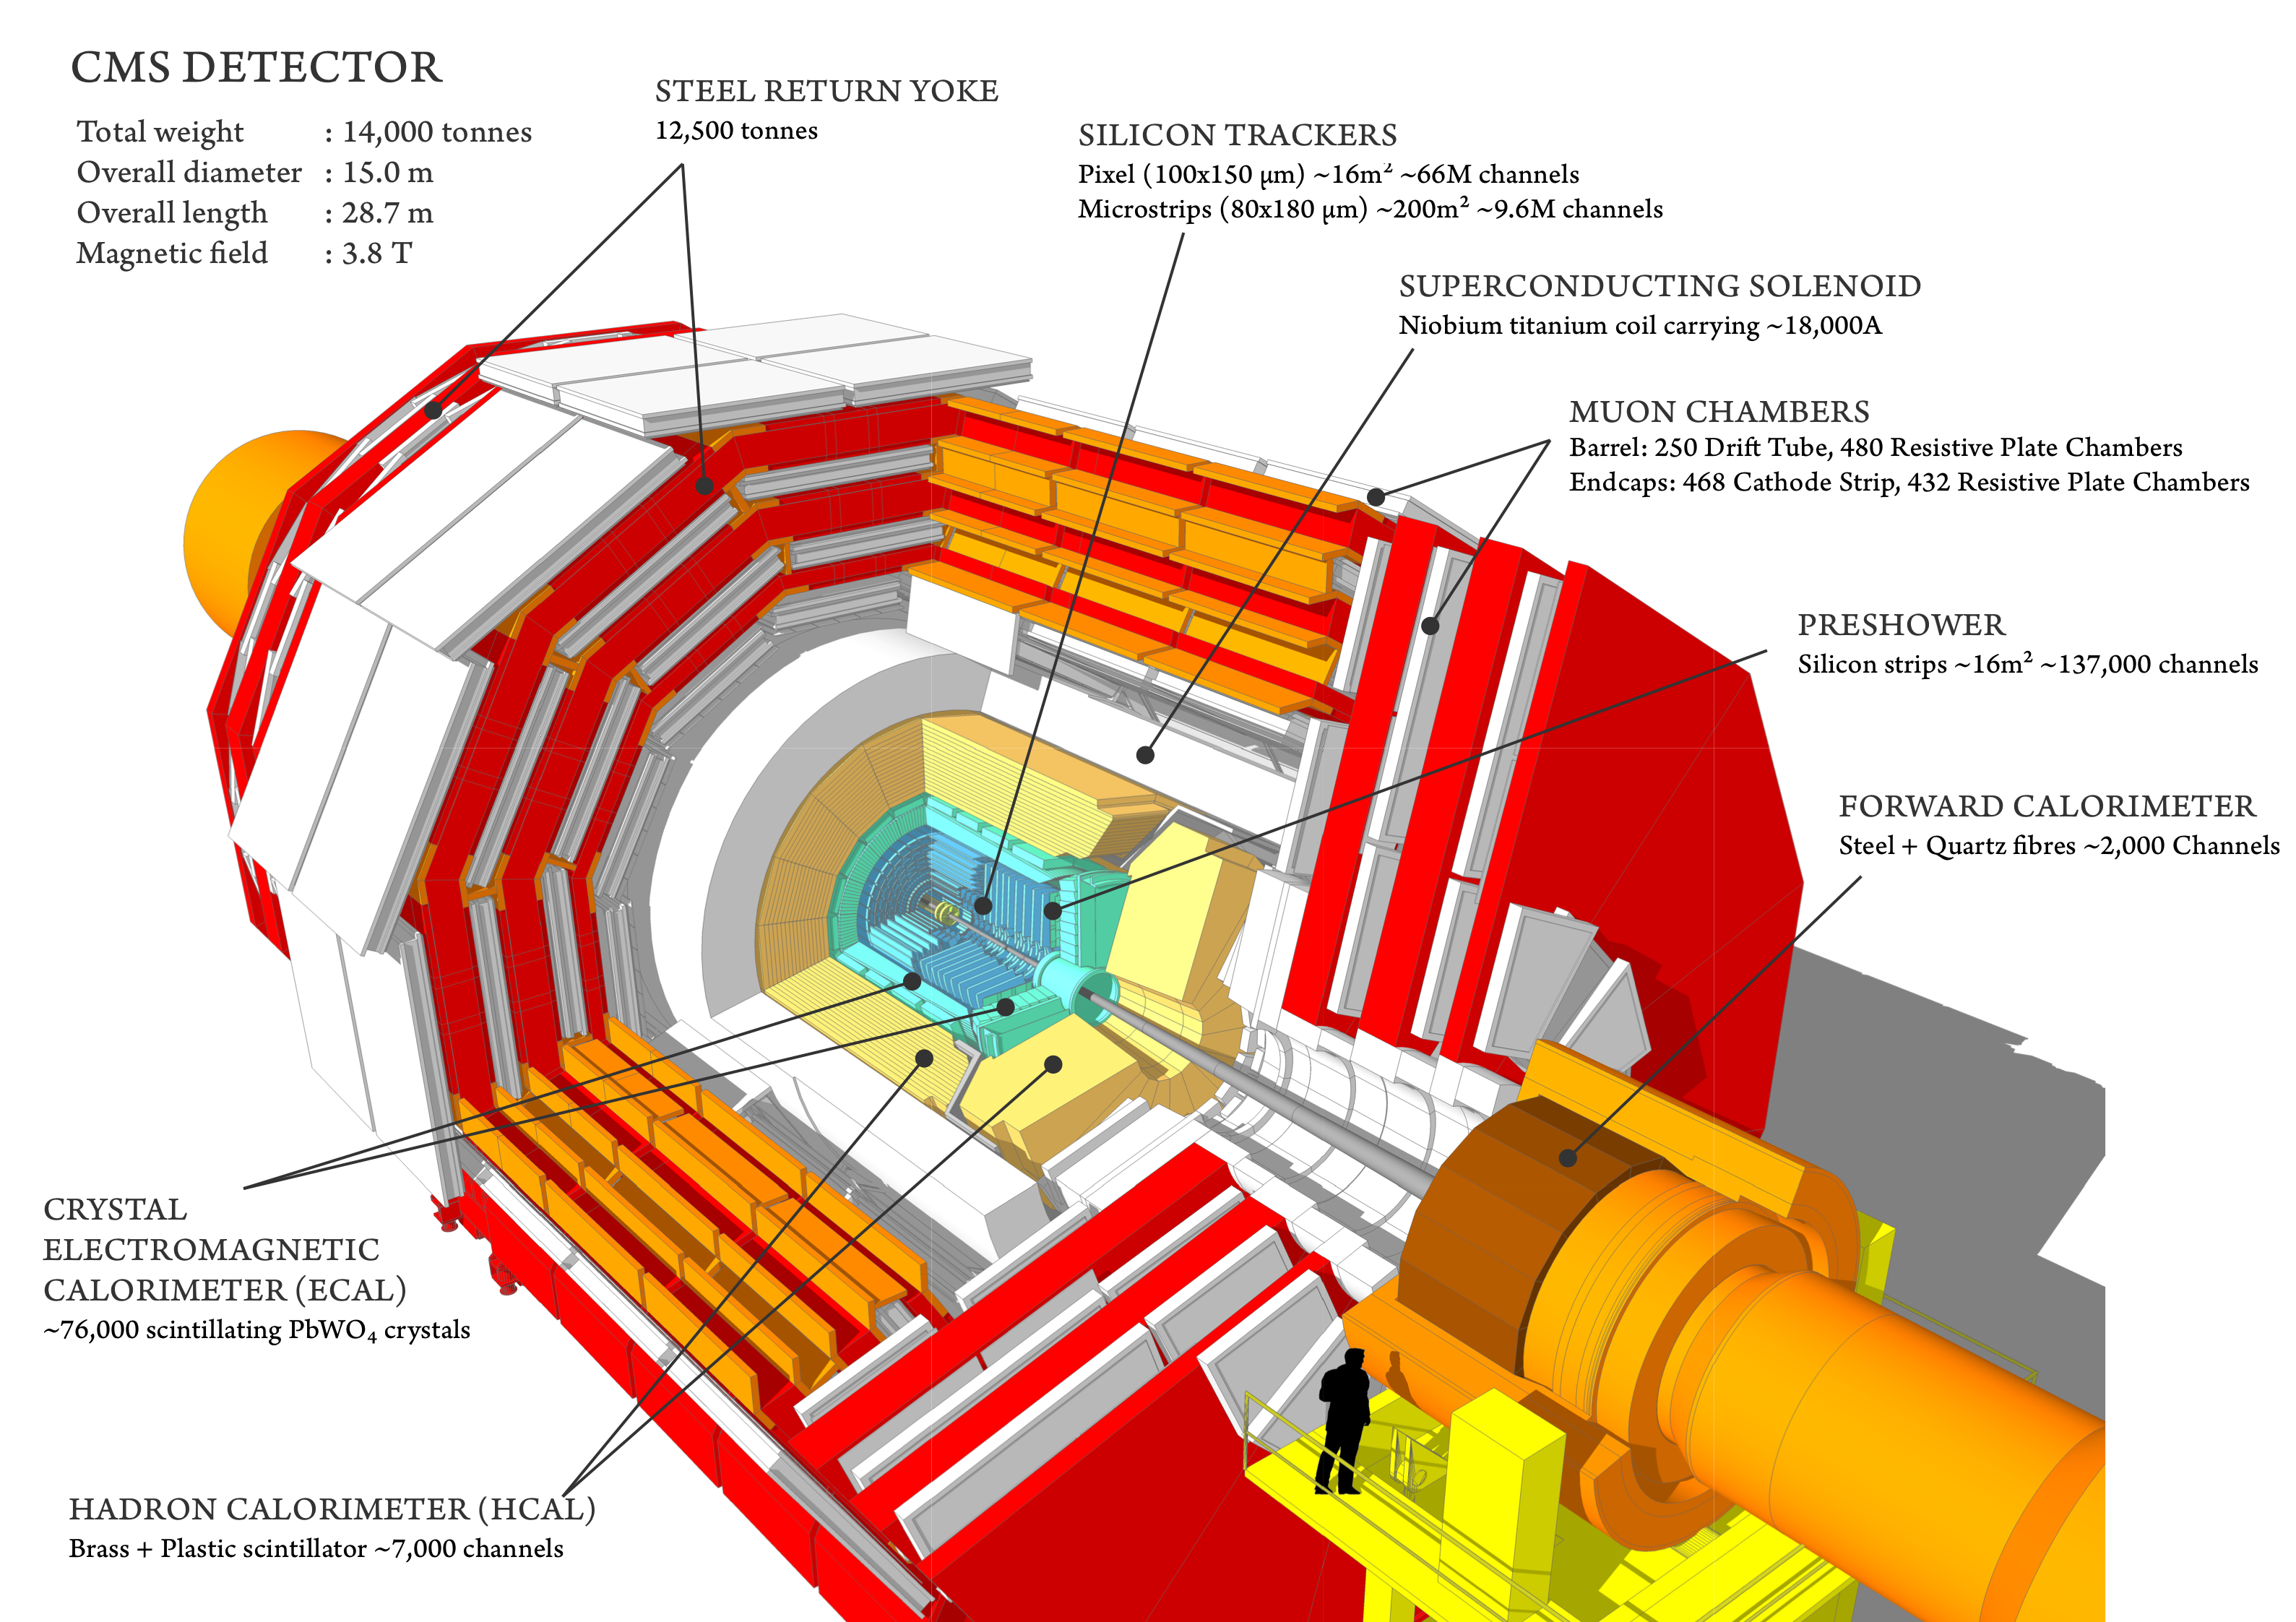
\includegraphics[width=0.9\textwidth]{figures/cms-cutaway.png}
\caption[Perspective view of the CMS detector, with cutaway showing
the many layers inside.]{Perspective view of the CMS detector, with
  cutaway showing the many layers inside \cite{websitecms}.}
\label{fig:cms:outside}
\end{figure}

The CMS detector was designed with a wide array of physics goals in
mind. Some of these goals included discovering the Higgs boson,
especially in decays to leptons or photons; discovering signs of
supersymmetry, if such signs exist; searching for extra
dimensions; and conducting precision tests of the predictions of the
Standard Model \cite{tdr}.
These and other goals had to be balanced against practical
constraints, such as budget, durability, and ease of readout. The
detector that resulted from the convergence of these factors is
described in detail in Sections
\ref{ssec:cms:components:magnet}-\ref{ssec:cms:components:muon}.

\subsection{Coordinates}
\label{ssec:cms:coordinates}

% Insert pictures that show detector coordinates, if possible

Before we can understand the design of the CMS detector, or the
physics it studies, we must assign a coordinate system to the detector.
Because the beam pipe has cylindrical symmetry, the CMS detector is
similarly cylindrical. It is shaped like a giant barrel wrapped around
the beam pipe, some 5 stories tall and wide, and 7 stories
long. The central part of the detector is actually referred to as the
\emph{barrel}, and the two plugs that cap off either end of the barrel
are known as the \emph{endcaps}.

The coordinate system attached to the detector may be seen in
plots throughout this Section. The longitudinal axis running down the
center of the beam pipe is defined to be the $z$-axis. The $+z$
direction points counterclockwise along the LHC, and the $-z$
direction clockwise. If we consider a circular
cross-section of the detector, as depicted atop Figure
\ref{fig:cms:wedge}, the radial coordinate $r$ expresses distance out from
the center, and the azimuthal angle is labeled $\phi$.

Because the proton beams are compressed and stabilized in the
transverse plane before they enter the collision area, we expect
that the system of two colliding protons has no net momentum
transverse to the beam pipe, i.e. in the $r$ direction. We can
therefore expect the total \emph{transverse momentum} (or $p_T$) of
the collision products to be zero. However, because the individual
partons inside a proton have constantly-changing momenta, we cannot
know the total longitudinal momentum ($p_z$) of the pp
collision. Because the total $p_T$ of the system is known a priori,
but $p_z$ is not, we consider the $p_T$ of particles almost
exclusively, and seldom spare a thought for $p_z$.

Because particle collisions take place near the
origin of the detector, it
is often helpful to describe the trajectories of particles in terms of
a sort of angle that they make in the $r-z$ plane. We could use the
polar angle $\theta$ from spherical coordinates. But in a world of
particles moving at relativistic speeds, we will often need to boost
between different reference frames, and $\theta$ becomes
cumbersome. Physicists came up with a more useful coordinate, which
they termed \emph{rapidity}. In collider physics, the rapidity, $y$,
of a particle is given by:
\begin{equation}
\label{eq:cms:rapidity}
y = \frac{1}{2} \ln \frac{E+p_z}{E-p_z}
\end{equation}
This coordinate has the advantage that
the rapidity difference $\Delta y$ between two particles is Lorentz
invariant--it remains the same no matter what reference frame it is
measured in.

Rapidity will be used to define other variables in Section
\ref{ssec:afb:variables}, but on the whole, it turns out to be not
very convenient, because it requires us to know the energy of the
particle. So physicists have devised a related quantity that behaves
somewhat better, calling it \emph{pseudorapidity}. The pseudorapidity,
$\eta$, of a moving particle is defined by
\begin{equation}
\label{eq:cms:eta}
\eta = -\ln \left[ \tan \left( \frac{\theta}{2} \right) \right]
\end{equation}
This coordinate depends only on the polar angle, not the energy, of a
particle. And like its cousin, the pseudorapidity difference $\Delta\eta$
between two particles is also a relativistic invariant. In fact, at
velocities approaching the speed of light, rapidity and pseudorapidity
become equal to one another. $\eta$ is used widely in collider
physics, even to the extent that parts of the CMS detector are
referred to by their ($\eta, \phi$) coordinates. Thus, you will see
labels employing the $\eta$ coordinate in Figures
\ref{fig:cms:tracker}, \ref{fig:cms:ecal}, \ref{fig:cms:hcal}, and
\ref{fig:cms:muon}.

We have established that differences $\Delta \eta$ in pseudorapidity
are invariant under Lorentz boosts along the $z$-axis. So too are
differences $\Delta \phi$ in the azimuthal angle, because $\phi$ is
measured transverse to the $z$-axis. So particle physicists often
use a 3-dimensional ``angle'' $\Delta R$, defined by:
\begin{equation}
\Delta R^2 = \Delta \eta^2 + \Delta \phi^2
\end{equation}
This not-quite-an-angle will be used in this and subsequent chapters
to measure the separation between two objects, and to define cones
around single objects, in a relativistically invariant way.

% CMS wedge diagram
\begin{figure}[htb]
\centering
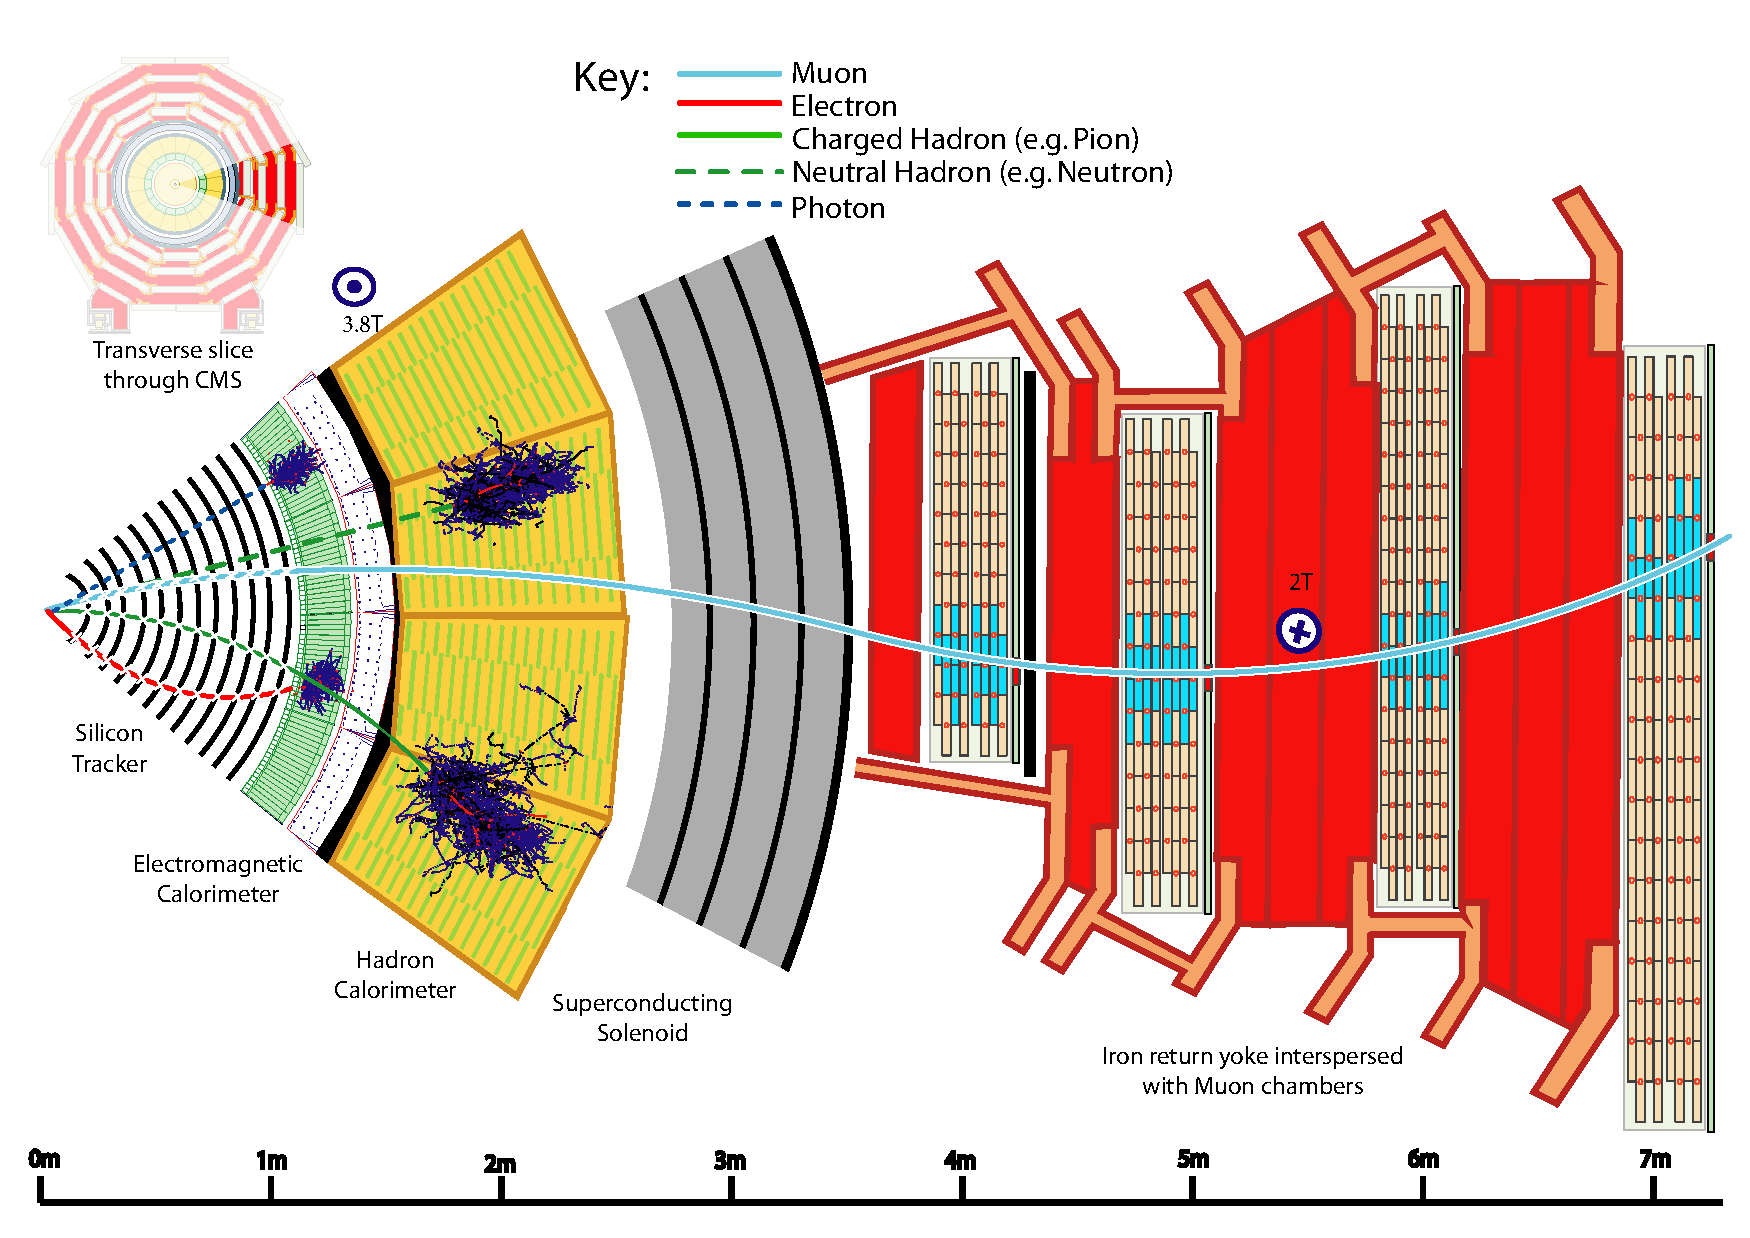
\includegraphics[width=0.9\textwidth]{figures/cms-wedge.pdf}
\caption[Diagram showing particles interacting with a typical
cross-sectional wedge of the CMS detector.]{Diagram showing particles
  interacting with a typical cross-sectional wedge of the CMS detector
  \cite{particleflow}.}
\label{fig:cms:wedge}
\end{figure}

\subsection{Superconducting Solenoid}
\label{ssec:cms:components:magnet}

Figure \ref{fig:cms:wedge} shows a small cross-sectional wedge
of the detector, and demonstrates how each of the components
contributes to measurements of the particles produced in the
collisions.

The defining feature of CMS, which gives rise to the 'S' in its name,
is the superconducting solenoid. This component is a large
electromagnet; it is made from superconducting niobium-titanium
material, taking the form of a giant coil 12.9m long and with an inner
bore of 5.9m \cite{tdr}. When cooled to about 4 Kelvin using liquid helium,
the magnet can generate a longitudinal magnetic
field of up to 4T inside the solenoid, though in practice we run it at
3.8T to help it last longer. The return field outside the
solenoid is lower, and is not uniform \cite{accelexper}.

The purpose of this magnet is to bend the trajectories of particles
passing through the detector. The tracker and the muon system
(described below) can measure the radius of curvature of a track, from
which we can determine how much momentum the particle was
carrying. The strength of the magnetic field was chosen based on
the requirement that the CMS detector be able to determine the charge
of a muon carrying 1 TeV of momentum \cite{tdr}.

\subsection{Inner Tracker}
\label{ssec:cms:components:tracker}

The innermost component of the detector, wrapped immediately around
the beam pipe, is the inner tracker. This component is made of several
layers of silicon sensors. Every time a charged
particle passes through a layer of silicon, it creates a blip of
electrical current in the silicon that can be read out
electronically. We can ``connect the dots'' to reconstruct the path
the particle took. Because of the magnetic field inside the detector,
charged particles will have curving trajectories. Using the tracker,
we can measure the radius of curvature of these tracks, and thus
determine the momentum of the particle that created the
tracks. Because the magnetic field is only in the z-direction, we can
only measure the $p_T$ of the charged tracks, not the
$p_z$. Importantly, neutral particles do not leave any hits in the
tracker, and thus their trajectories and momenta cannot be measured.

% Figure of the tracker geometry
\begin{figure}[htb]
\centering
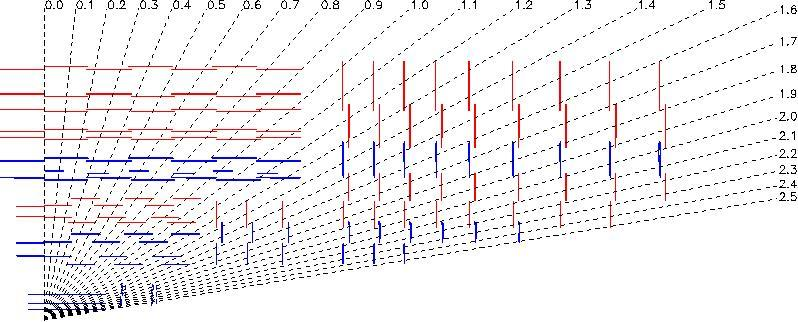
\includegraphics[width=0.9\textwidth]{figures/tracker.jpg}
\caption[One-quarter $(r,z)$ view of the layout of the CMS inner
tracker.]{One-quarter $(r,z)$ view of the layout of the CMS inner tracker \cite{tdr}.}
\label{fig:cms:tracker}
\end{figure}

Figure \ref{fig:cms:tracker} shows the geometry of the tracker as originally designed.
The innermost part of the tracker ($r \lesssim$ 10cm), where the tracks are densest,
consists of silicon pixels. At installation, there were three pixel
layers in the barrel and two in the endcaps. Each pixel is
100$\times$150 $\mu$m in size. At this scale, the expect occupancy of
a pixel was $10^{-4}$ per bunch crossing \cite{tdr}. The pixel tracker
was upgraded during the 2016/2017 winter shutdown, adding a fourth
pixel layer in the barrel and a third in the endcaps, while slimming
down the hardware that supports the functioning of the pixels
\cite{pixeltdr}.

The remaining layers of the tracker consist of silicon strips. In the
region $20 < r < 55$ cm in the barrel (Tracker Inner Barrel, TIB),
there are four layers of silicon
microstrips, with a size of at least 10 cm $\times$ 80$\mu$m. In the
Tracker Outer Barrel (TOB), defined by $r >$ 55cm, there are six
layers of microstrips with a size of no more than 25 cm $\times$
180$\mu$m. In the endcap regions, the Tracker Inner Disks (TID) sit
just outside the TIB, and consist of three layers of disks of
strips. The Tracker Endcaps (TEC) sit just outside the TOB, and
consists of nine disks of silicon strips. These various layers provide
tracker coverage out to $|\eta| \approx 2.5$.

The electrical impulses produced in the silicon pixels and strips are
read out by ``APV25'' chips that amplify and process the signals. The
signals are then passed out of the detector using optical cable, and
further processed in hardware outside the detector itself
\cite{tdr}. Additional hardware circulates a refrigerant liquid that
maintains the silicon sensors at a temperature no higher than
$-10^\circ$ C \cite{accelexper}. The materials and geometry of the
original tracker are chosen to minimize the amount of energy absorbed
from particles as they pass through.

The performance of the inner tracker has been measured using both
muons and pions. The $p_T$ resolution for muons ranges from about 0.5
- 2.0\%, depending on $p_T$ and $\eta$. The efficiency of
global muon track reconstruction is generally around 99\%. For pions,
the global track resolution is somewhat less, ranging from 85-95\% for
100 GeV pions and 75-90\% for 1 GeV pions \cite{tdr}.
% Consider pulling some of the resolution plots

\subsection{Electromagnetic Calorimeter (ECAL)}
\label{ssec:cms:components:ecal}

Just outside the tracker, the next component in the CMS
detector is the electromagnetic calorimeter, or ECAL. The purpose of
this device is to measure the energy of electromagnetic particles
(electrons and photons) produced in collisions. The ECAL consists
of a giant array of lead tungstate (PbWO$_4$) crystals; when struck by
electromagnetic particles, these crystals scintillate with a
pale blue light that can be read out by optical sensors. The amount of
light gives us a measure of how much energy the particle was
carrying. In addition, the pattern of energy deposition in the
crystals can provide information useful in particle
reconstruction.

Lead tungstate has a number of properties that make it an ideal
material to use in the ECAL. For one thing, it is quick to read
out: lead tungstate crystals can release 80\% of their scintillation
photons in the 25ns window between bunch crossings. In
addition, lead tungstate is highly resistant (``hard'') to the high
levels of radiation emitted by the collisions, tolerating a total
absorbed dose of up to 10 Mrad (100 kGy). But perhaps most importantly,
lead tungstate allows the ECAL to be built relatively compactly,
because the material has a short radiation length ($X_0$) and
Moli\`{e}re radius ($R_M$).

Radiation length and Moli\`{e}re radius are two properties that
describe a material's ability to absorb electromagnetic energy. When
an electron passes into a material, the radiation length is the
characteristic distance over which that electron will lose all
but 1/$e$ of its energy. To put it mathematically:
\begin{equation}
\label{eq:cms:ecal:radlength}
E(x) = E_0 \cdot e^{-x/X_0}
\end{equation}
It is also equal to 7/9 of the mean free path for pair production by
photons \cite{pdg}. So the shorter the radiation length for a
material, the shorter the distance needed for electromagnetic
particles to be stopped and their energy absorbed. Lead tungstate has
a radiation length $X_0 = 0.89$ cm \cite{tdr}. Similarly, the
Moli\`{e}re radius governs the absorption of energy in the direction
transverse to the particle's trajectory. It is the characteristic
lateral distance over which 90\% of an EM shower's energy will be
contained. So materials with a shorter Moli\`{e}re radius will have on
average a smaller transverse shower size. For lead tungstate, $R_M =
2.2$ cm \cite{tdr}. These characteristic distances will play a role in
determining the size of the ECAL crystals.

% Diagram of ECAL layout
\begin{figure}[htb]
\centering
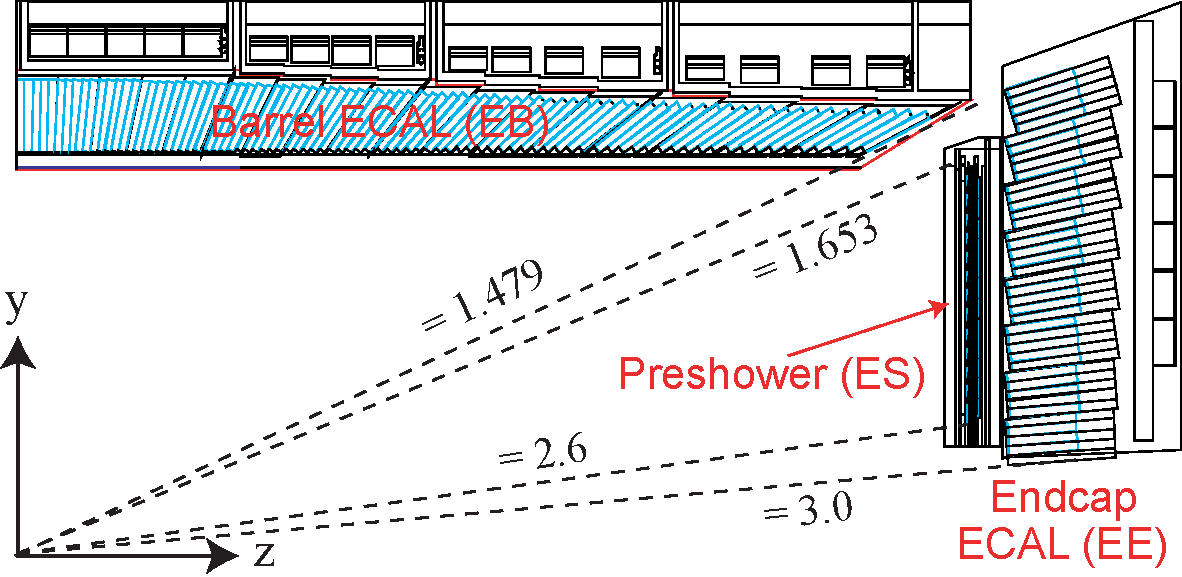
\includegraphics[width=0.9\textwidth]{figures/ecal-layout.pdf}
\caption[One-quarter $(r,z)$ view of the layout of the CMS ECAL.]{One-quarter $(r,z)$
  view of the layout of the CMS ECAL \cite{tdr}.}
\label{fig:cms:ecal}
\end{figure}

The ECAL is divided into barrel and endcap components.
These may be seen in Figure \ref{fig:cms:ecal}.
The PbWO$_4$ crystals are shaped like tapered rectangular prisms. In
the barrel region, they are 230 mm long, corresponding to 25.8 $X_0$,
and have front faces that are 22$\times$22 mm, corresponding to
1$\times$1 $R_M$. These dimensions ensure that very little EM energy
will escape out the back of the crystals, and that
about 94\% of a given shower will be contained in a 3$\times$3 array
of crystals. In the endcaps, the crystals are 220 mm long (24.7 $X_0$),
and have front faces of 28.6$\times$28.6 mm (1.3$\times$1.3 $R_M$).
The barrel section is composed of 36 ``supermodules''. Each
supermodule is an array of 85$\times$20 crystals, covering half the
barrel length and 20$^\circ$ in $\phi$. Each of the two endcaps is
composed of two half-circle structures called ``Dees''. Each dee holds
138 groupings of 5$\times$5 crystals (called``supercrystals'') plus
18 partial supercrystals. The endcaps are also fronted with preshower
detectors, whose purpose is primarily to study neutral pions produced
at high $\eta$. These preshower detecters are composed of lead
absorbers that initiate pion showering, and silicon strip detectors
that measure the size and shape of the shower. All told, there are
75,848 crystals in the entire ECAL, providing very fine spatial
granularity. As Figure \ref{fig:cms:ecal}
shows, ECAL coverage extends out to $|\eta|$ = 3.0. However, there is
a gap in coverage between the barrel and the endcaps. Electromagnetic
particles that fall into this ``crack'' will not be measured, a fact
that we must account for when attempting to reconstruct electrons and
photons \cite{tdr}.

Lead tungstate produces a blue-green scintillation light, peaking near
420mm. The amount of light produced in each crystal must be measured,
and the information digitized, in order to determine the energy of incident EM
particles. In the
barrel, scintillation photons are read out by silicon avalanche photodiodes (APDs)
stuck to the backs of each crystal. In the endcaps, vacuum
phototriodes (VPTs) are used for readout instead. These sensors feed
their signals to amplification and digitization hardware attached to
the CMS detector, and from there are sent to computing equipment
outside the detector volume \cite{tdr}.

The performance of the ECAL was measured using a controlled beam of
electrons. The measured energy resolution in groups of 3$\times$3
crystals is better than 1\% for electron energies above about 20 GeV \cite{tdr}.

\subsection{Hadron Calorimeter (HCAL)}
\label{ssec:cms:components:hcal}

Outside the ECAL but (mostly) inside the magnet lies the hadron
calorimeter, or HCAL. This component is designed to measure the energy
of hadronic particles produced in collisions. The HCAL is composed of
alternating layers of metal, used to absorb some of the incident
hadronic energy, and scintillating materials, used to measure the
hadronic energy deposited in the calorimeter. The HCAL thus has an
important role in measuring the energy of jets, as well as in
measuring pileup from secondary collisions in the event.

The power of materials to stop relativistic particles is described in
terms of the interaction length, $\lambda_I$. When a number of
particles are incident on some material, this parameter describes
the length over which all but a 1/$e$ fraction of those particles will
be absorbed. In other words:
\begin{equation}
\label{eq:cms:hcal:intlength}
N(x) = N_0 \cdot e^{-x/\lambda_I}
\end{equation}
So the shorter a material's interaction length, the shorter the
distance over which it will absorb incident particles.

The CMS HCAL is a \emph{sampling} calorimeter, meaning that it uses
different materials to produce the shower and to measure the
energy. Hadronic showering is induced by the absorber layers, most of
which are made of brass (70/30\% Cu/Zn). Brass
is used because it is relatively affordable, and also because it is
non-magnetic, and thus won't perturb the magnetic field inside the
detector. This particular brass alloy has an interaction length
$\lambda_I = 16.42$ cm. Stainless steel is also used as an absorber in places.
Interleaved with the absorber materials are layers of
scintillating material. Most of the scintillators are made of
radiation-hard plastic, either Kuraray SCSN81 or Bicron BC408, though
where extreme particle flux and radiation is an issue, quartz fiber is
used instead for its superior radiation hardness.

The HCAL is divided into four subcomponents: the barrel (HB), the
endcaps (HE), the outer calorimeter (HO), and the forward calorimeter
(HF). Each of these components operates on the same principles, though
the design of each differs slightly. These components are all cleverly
overlapped to avoid any cracks like that of the ECAL. The arrangement
of the components is showin in Figure \ref{fig:cms:hcal}.

% Plot showing HCAL layout
\begin{figure}[htb]
\centering
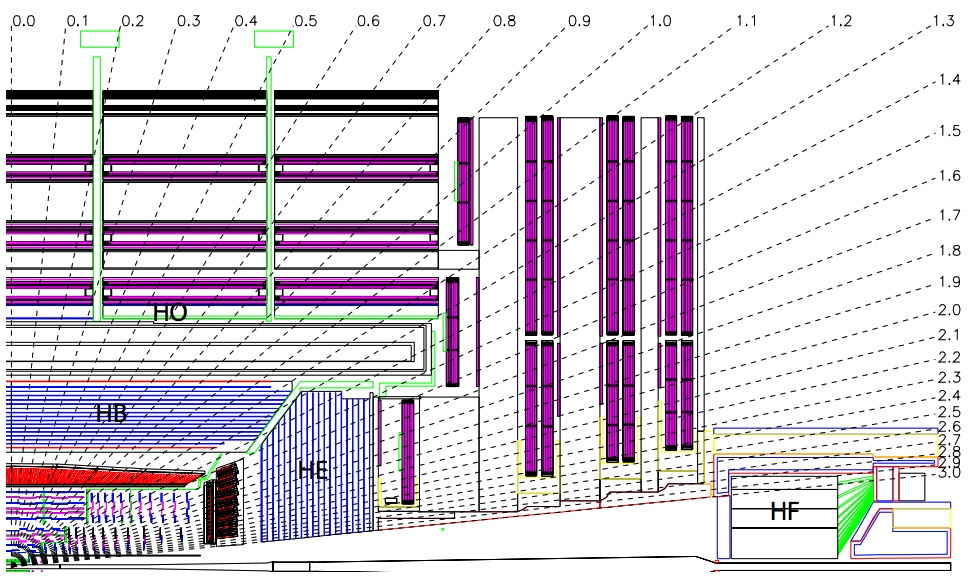
\includegraphics[width=0.9\textwidth]{figures/hcal-layout.jpg}
\caption[One-quarter $(r,z)$ view showing the layout of the HCAL components within the
CMS detector.]{One-quarter $(r,z)$ view showing the layout of the HCAL components within the
  CMS detector \cite{cms}.}
\label{fig:cms:hcal}
\end{figure}

The barrel covers the range $|\eta| <$ 1.3. The absorber material in
the HB is segmented into 36 wedges; each wedge encompasses half the
length of the HB and 20$^\circ$ in $\phi$. There are 16 layers of
absorber material in each wedge; the innermost and outermost layers are
made of stainless steel, for strength, and the middle 14 layers are
brass. The total thickness of these absorber layers is 5.82
$\lambda_I$ at $\eta$ = 0, increasing to 10.6 $\lambda_I$ at $|\eta|$
= 1.3. Within each wedge, the scintillating material is further
divided into segments of size 0.087$\times$0.087 in $(\Delta\eta,\Delta\phi)$
space, providing fine granularity. The innermost layer of
scintillating material in the HB is Bicron BC408, and the remaining 16
layers are Kuraray SCSN81 \cite{accelexper}.

The endcaps cover the regions 1.3 $< |\eta| <$ 3.0, and use the same
absorber and scintillator materials as the barrel, with one exception:
stainless steel is only used as the outer absorber layer, to
prevent any magnetic interference inside the magnet bore. The
scintillators are divided into segments of size 0.087$\times$0.087 in
$(\Delta\eta,\Delta\phi)$ space for $|\eta| <$ 1.6, and approximately
0.17$\times$0.17 for $|\eta| \geq$ 1.6. The total thickness of the
endcaps (including attached ECAL dees) is about 10 $\lambda_I$
\cite{accelexper}.

The outer calorimeter is designed to augment the stopping power of the
HB and the EB, and covers the region $|\eta| <$ 1.3. It consists of
tiles of Bicron BC408 scintillator embedded in the iron yoke that
gathers the returning magnetic field outside the solenoid. Thus the HO
actually uses the solenoid material itself as an absorber.
Following the shape of the return yoke, the HO is divided into 5 rings
along the $z$-axis, each of which has 12 sectors in $\phi$. There are
gaps between the rings and in some azimuth sectors for the cryogenic
and power lines that supply the magnet. The scintillator tiles roughly
follow the 0.087$\times$0.087 segmentation of the HB, within the
constraints of the yoke geometry \cite{accelexper}.

The forward calorimeter is located in the region 3.0 $< |\eta| <$
5.2. This area receives an extremely high flux of particles due to its
small angle with respect to the beamline. As such, this component
must be considerably more radiation hard than any other part of the
HCAL. To meet this requirement, the HF uses quartz fibers with polymer
cladding as its measuring material, and reads out Cherenkov light rather than
scintillation light. Each end of the HF is composed of stainless steel
absorbers arranged in 18 azimuthal wedges, each of which is penetrated
by quartz fibers that run parallel to the beamline. Some of these
fibers only penetrate partway through the steel plate, allowing the HF to
differentiate between electromagnetic and hadronic showers based on
penetration depth. The fibers form towers of size 0.175$\times$0.175
in $(\Delta\eta,\Delta\phi)$ space \cite{accelexper}.

The scintillation light from the plastic tiles is read out by
Kuraray Y-11 wavelength-shifting (WLS) fibers. These fibers are embedded
into the tiles themselves. Once outside the tiles, the WLS fibers are
spliced to clear optical fibers that send the light to hybrid
photodiodes for electronic processing. The Cherenkov light from the
quartz fibers is transmitted to air-core light guides, which carry the
light through layers of radiation shielding to photomultiplier tubes
outside the shielding \cite{accelexper}.

% Resolution/performance?
   % Figure 1.8 apparently shows that JER as a function of ET is similar in all parts of the HCAL
   % MET resolution function is given in 1.5.4.5
   % May need to see TDR chapter 11? (This according to 1.5.4.5).
   % See also TDR 5.4?

\subsection{Muon System}
\label{ssec:cms:components:muon}

The outermost component of the CMS detector is the muon system. The
strong penetrating power of muons allows us to place this system
outside all the other layers without fear that the muons will be
absorbed en route. As its name suggests, the muon system is
responsible for measuring the momentum of muons as they fly away from
the collision point. It employs three different gas-and-electrode
technologies to reconstruct the trajectories of muons, from which
momentum can be inferred. These trajectories can be combined with
measurements from the tracker for greater precision.

% Layout of the muon system
\begin{figure}[htb]
\centering
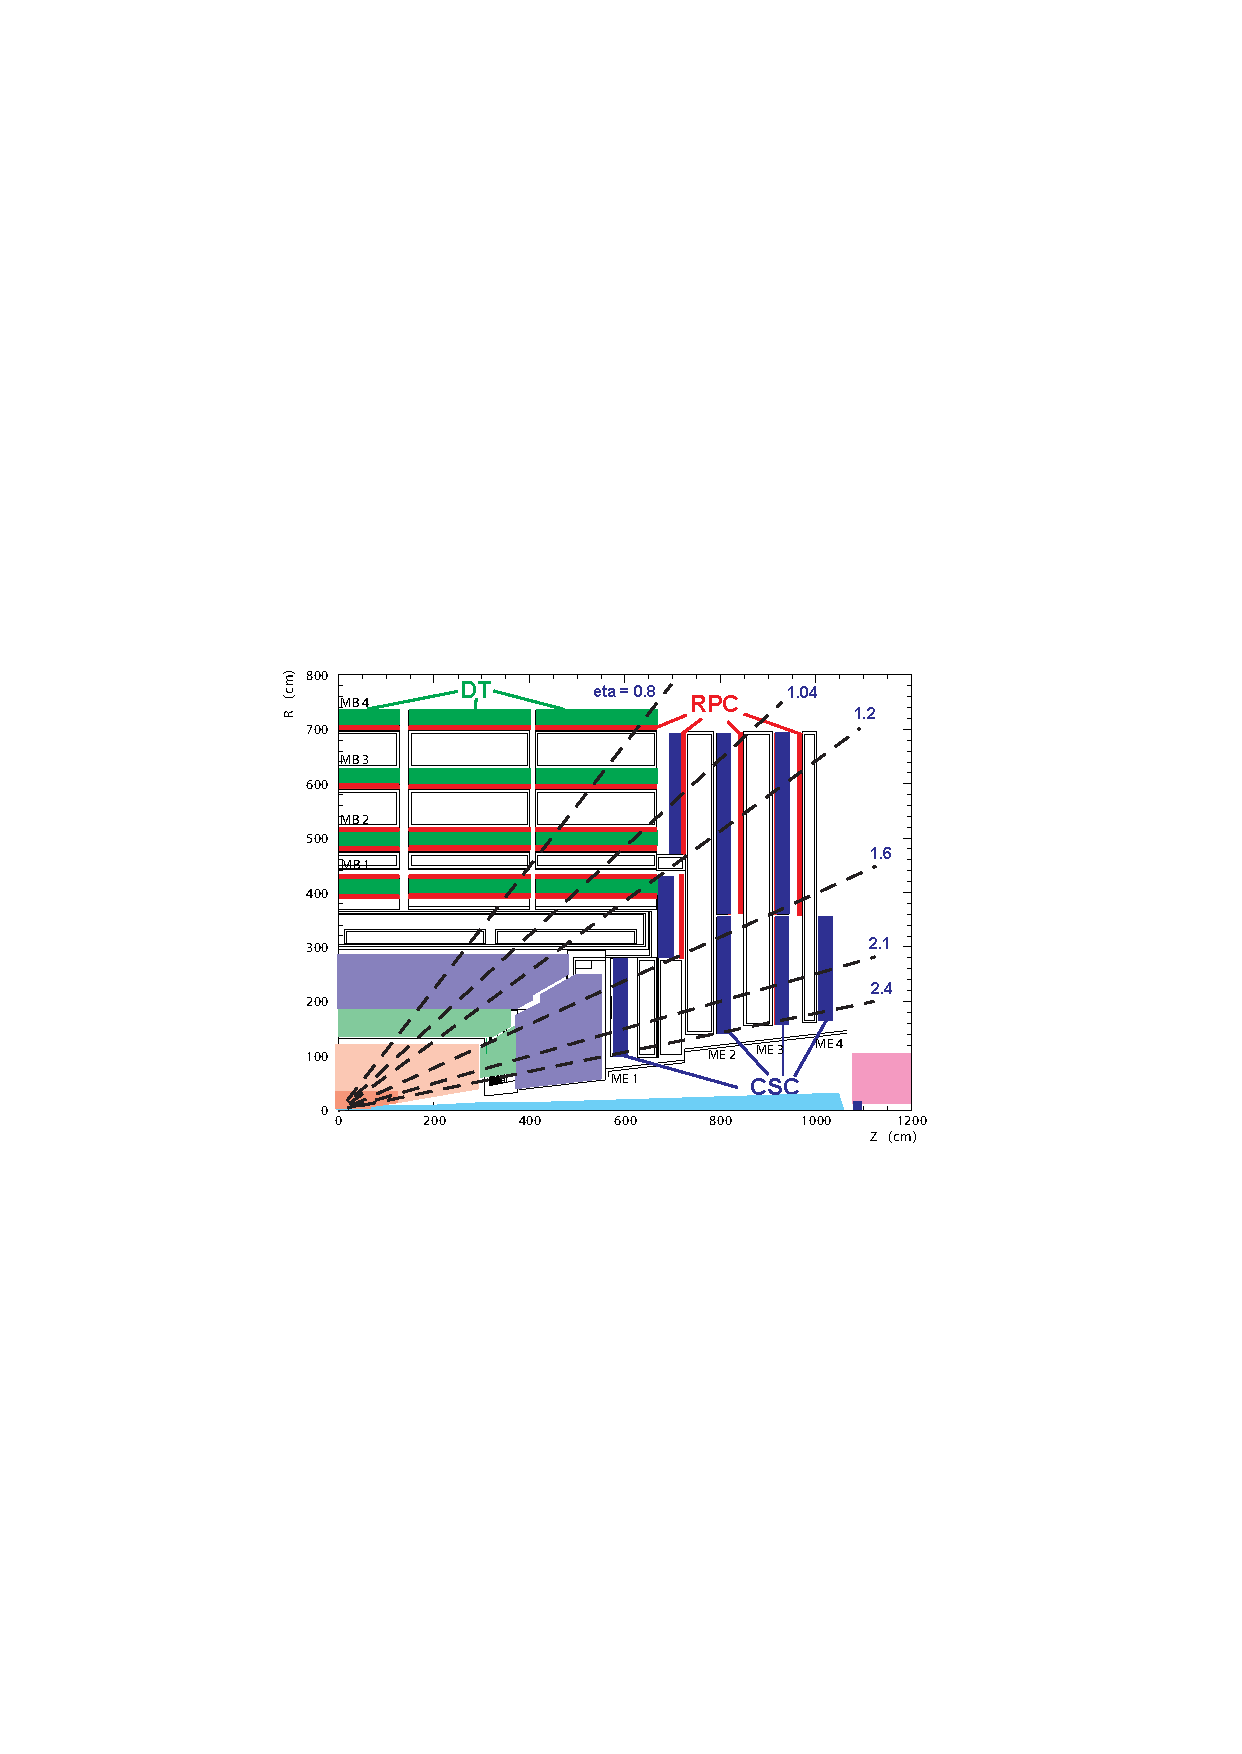
\includegraphics[width=0.9\textwidth]{figures/muon-layout.pdf}
\caption[One-quarter $(r,z)$ view of the layout of the CMS muon
system.]{One-quarter $(r,z)$ view of the layout of the CMS muon system
  \cite{tdr}.}
\label{fig:cms:muon}
\end{figure}

The layout of the muon system is presented in Figure \ref{fig:cms:muon}.
Like many other components, it is divided into barrel and endcap
regions. The barrel region detects muons using a combination of drift
tubes (DTs) and resistive plate chambers (RPCs), whereas the endcaps use cathode
strip chambers (CSCs) and RPCs. All three of these technologies detect
muons by the trail of ionization the muons leave after passing through a gas. The
liberated electrons will be attracted to positively charged
electrodes, and the ions to negatively charged electrodes. When
electrons and ions hit the electrodes, they produce an electrical
signal that is read out, and timing information
is used to tell how far along the electrode the impact occurred.

The drift tubes are long, thin chambers filled with a mixture of 85\%
Ar and 15\% CO$_2$ gases, and with a positively charged wire running
down their centers. Drift times in these chambers are a maximum of 380
ns. These tubes provide 1D position measurements, but multiple layers
may be stacked at right angles to
provide 2D measurements. These devices are used because they are precise
and inexpensive, and can function well in the muon barrel, where the
particle flux and magnetic field are both low
\cite{accelexper,websitedt}. The cathode strip chambers are planar
chambers filled with a mix of 40\% Ar, 50\% CO$_2$, and 10\%
CF$_4$. They contain positively charged wires running in
one direction, and negatively charged strips running perpendicularly,
providing native 2D position measurements. CSCs are employed in the
endcap because they are precise, moderately fast ($<$ 225 ns), and can operate
in the high magnetic fields at the fringes of the solenoid
\cite{accelexper,websitecsc}. Resistive plate chambers are planar
chambers filled with a mixture of 96.2\% C$_2$H$_2$F$_4$, 3.5\%
$i$C$_4$H$_{10}$, and 0.3\% SF$_6$. They have a positively charged
plate on one face, and a negatively charged plate on the
opposite face. Electrons are actually detected by metal strips just outside
the chambers. RPCs are used to supplement the DTs and CSCs
mainly for their 1 ns timing resolution; their spatial
resolution is not as fine as the DTs or the CSCs
\cite{accelexper,websiterpc}. The signals from these subsystems are
processed in electronics both within the detector volume and outside it.

The barrel section of the muon system, covering $|\eta| <$ 1.2, is
interleaved with the iron return yokes, structures that concentrate
the magnetic field exiting the solenoid and return it around to the
other end. As such, the muon barrel follows the geometry of the
yokes. The return yokes consist of five rings that are about 2 meters long
and divided into 12 sectors in $\phi$. As Figure \ref{fig:cms:muon} shows,
the DTs and RPCs are stacked in four layers, or \emph{stations}. These
are offset in $\phi$ so that all muons will pass through at least
three stations. The three innermost stations contain 12 planes of DTs, 8 of
which provide $(r,\phi)$ measurements, and 4 of which provide $z$
measurements. The outer station lacks the $z$ measuring planes. The
inner two stations are coupled to two RPCs each, and the outer two
stations have one RPC each. With this geometry, each individual
station can provide position measurements with a precision of better
than 100 $\mu$m in space and about 1 mrad in $\phi$ \cite{tdr}.

The endcap muon system covers the range 0.9 $< |\eta| <$ 2.4. The
CSCs are arrayed in four layers of disks, with each disk being made up
of several trapezoidal chambers 10 or 20$^\circ$ wide in $\phi$,
arranged in concentric rings. Each chamber contains 6 gas gaps and
electrode grids. There are 36 chambers in each ring, except the
centermost rings of stations 2-4, which have only 18 chambers. The
CSCs provide a spatial resolution of about 200 $\mu$m and an angular
resolution in $\phi$ of about 10 mrad \cite{tdr}. During Run I, the
first three disks had RPCs attached to all but the central ring; for
Run II, the outer CSC ring of disk 4 was added, and was instrumented
with attached RPCs.

% Anything I want to say about cosmics?

\section{Triggers}
\label{sec:cms:triggers}

As previous sections have described, the LHC collides protons at a
rate of 40 million collisions per second. However, the number of
collisions per second that can actually be recorded is ultimately
dictated by the medium used to store the data. Magnetic disk drives
are prohibitively slow for our uses, while solid-state
drives are both prohibitively slow and expensive. So in particle
physics, we store our data
on magnetic tape (like one might find in a video or audio
cassette). The data recording system allows us to keep only about one
of every 100,000 events.

Fortunately, this constraint is less harmful than it might seem,
because not every event is worth saving. Even with the
considerable beam focusing power of the LHC, most bunch crossings only produce
near-misses or grazing contact between protons. True head-on pp
collisions, producing particles with a high transverse component to
their momentum, are somewhat rare. Thus we can reach a manageable threshold of
$<$1000 events per second using a system of ``triggers'' to store only
events where interesting physics is taking place.

The first stage of the trigger system is the Level 1 trigger
(L1). The L1 trigger is integrated directly into the detector
hardware, and does not use any computational resources. It
is tripped by basic signatures such as ionization tracks in the muon system, ECAL
deposits consistent with electrons or photons, HCAL deposits
consistent with jets, and a few others. This trigger system is able to
make extremely fast decisions, and outputs events at a rate of 100
kHz \cite{trigger}.

Events passing the L1 triggers are handed off to the second trigger
stage, called the high-level trigger (or HLT). This stage uses
banks of commodity computers running physics reconstruction
software to make a much more sophisticated determination of what
physics objects are present in the event. Thanks to this more
detailed reconstruction, the HLT allows one to trigger on a wide
variety of signatures with a high degree of specificity. The HLT
outputs events at an average
rate of about 400 Hz; these are then stored for eventual use in
physics research \cite{trigger}.

The use of these trigger systems can create certain difficulties
that must be compensated for during physics analysis. For one, the
triggers are not perfectly \emph{efficient},
meaning they miss some fraction of the events they are intended to
trigger on. For example, a trigger designed to select events
containing muons with $p_T >$ 17 GeV might only select 98\% of those
target muons, and this fraction might even vary with the muon
$p_T$. This effect must be measured, and accounted for when we compare
our data against theoretical predictions. Another problem is that
certain very common signatures (e.g. a single electron) occur more
frequently than the triggers can handle. To cope with this flood of
events, we may have to program the trigger to record only every
$n^\text{th}$ event, and weight that event to count $n$
times. This is called \emph{prescaling} the trigger. Because
weighting up prescaled events reduces our statistical precision, we
try to use un-prescaled triggers whenever possible.

\section{Reconstruction and Identification}
\label{sec:cms:recoandid}

In order to do meaningful particle physics, we must translate the
output from the CMS detector into a picture of what particles and
objects are present in the event. This is the process of event
reconstruction (``reco'') and particle identification (``ID''). There
are any number of possible algorithms for converting detector
signatures into particles. The CMS Collaboration performs its basic
reconstruction using a system called particle flow (PF).

\subsection{Particle Flow}
\label{ssec:cms:reco:pf}

The particle flow algorithm attempts to associate all of the detector
readings with particles or physics objects. It begins by
reconstructing all the tracks, calorimeter energy clusters, and
vertices in the event. Then, using this information, the algorithm
iteratively attempts to reconstruct all the particles and physics
objects in the event using all available detector information. It
starts with the easiest objects to identify (muons); once all the
muons in an event are reconstructed, the corresponding detector
signatures are removed, and the next easiest identifications are
attempted, and so on. Each successive ID step uses only the
information that has not been consumed by a previous step. Some
postprocessing is performed at the end \cite{particleflow}.

\subsubsection{Charged Tracks and Vertices}
\label{sssec:cms:pf:trackvert}

As a prelude to reconstructing particles, the PF algorithm begins by
reconstructing tracks from the pixel and strip hits in the inner
tracker. These tracks are reconstructed using a sophisticated method
based on Kalman filtering, which is described in References
\cite{kalman1} and \cite{kalman2}. In short, this method attempts to
connect hits in successive layers and fit them to a helical
trajectory. The method places tunable constraints on the minimum
number of sequential hits required, the maximum number of missing
``expected'' hits, and other quantities to ensure that tracks may be
reconstructed to a desired level of quality.

Once all the tracks in the event are identified, they must be grouped
into vertices. A vertex is a spot where a proton-proton interaction
took place and produced some particles. Vertices are reconstructed by
extrapolating tracks backward to see where they originated from, and finding
spots where several tracks intersect. As mentioned previously, a
single event may contain multiple proton-proton interactions, and thus
multiple vertices. The vertex associated with the highest sum of
squares of track $p_T$ is known as the \emph{primary vertex}; when
analyzing an event, we only consider particles emanating from the
primary vertex. Any other vertices are called secondary, and the
particles originating from them are considered pileup.

\subsubsection{Calorimeter Clusters}
\label{sssec:cms:pf:caloclusters}

The next step before reconstructing particles is to group the energy
deposits in the ECAL and HCAL into clusters. The clustering process
is important for differentiating between electrons and photons, and
between charged hadrons and neutral hadrons. Each cluster begins with
a \emph{seed}--a calorimeter cell whose measured energy is above some defined
threshold. From the seed, a cluster is formed by
recursively adding in any adjacent cells with sufficient energy, and
then fitting the energy distribution with a 2D Gaussian. Separate
calibrations are applied in the endcap and barrel of each calorimeter,
to account for the differences in geometry and detector layout between
the regions \cite{particleflow}.

\subsubsection{Muons}
\label{sssec:cms:pf:muons}

Once the tracks, vertices, and clusters have been formed, the particle
flow algorithm attempts to reconstruct any muons in the
event. Muons are the natural starting point because their signature is
very distinctive and usually quite clean. The ideal muon is made by joining a
track in the muon system with a track in the inner tracker that lines
up appropriately. A muon that comes directly from the collision is expected
to have a low value for its \emph{isolation}, a measurement of how
much energy and momentum is found within a cone of radius $\Delta R <$
0.3 around the hypothesized muon track. A muon
that uses both tracker and muon-system information is known as a
\emph{global} muon. Sometimes it may also be possible to reconstruct
\emph{tracker-only} muons or \emph{standalone} muons, which use only
information from the inner tracker, or the muon system,
respectively. Once a muon candidate is identified, the associated
tracks are removed from consideration in future identification
steps \cite{particleflow}.

\subsubsection{Electrons and Photons}
\label{sssec:cms:pf:egamma}

Electrons and photons are processed in the same step because the
identification of both particles relies on ECAL energy deposits. A
potential electron starts out as a charged track that matches up with
a suitable ECAL energy deposit; a photon is suspected when there
is an ECAL deposit that has no corresponding track. To solidify the
identification, a number of further identification criteria are
checked in each case.

The shape of the ECAL energy deposit is a key clue used in identifying
electrons and photons. As they pass through the tracker, electrons
tend to produce \emph{bremsstrahlung}, a shower of photons that
radiate off as the electron's path bends. These photons tend to then
convert into electron-positron pairs, which may produce further
bremsstrahlung, and so on. This shower, emitted along the curved
trajectory of electrons, means that electrons often appear in the ECAL
as a pronounced energy deposit with a long tail of clusters in the $\phi$
direction. Photons, by contrast, are not bent by the magnetic field,
and thus tend to create rounder energy deposits wherever they strike
the ECAL.

A number of other variables are also used in identifying electrons and
photons. For instance, electrons and photons shower somewhat
differently when they strike the ECAL crystals, giving rise to a
number of variables describing the transverse shower shape. It is also
worth pointing out that decaying
hadrons can produce photons, so in order to
claim an electron or photon originated in the hard collision, its
associated ECAL deposits must not overlap large HCAL energy
deposits. Photons are also required to be isolated \cite{particleflow}.

\subsubsection{Hadrons}
\label{sssec:cms:pf:hadrons}

Once isolated muons, electrons, and isolated photons are removed from
the event, the only particles left to identify are charged and neutral
hadrons. At this step, particle flow also attempts to reconstruct
non-isolated photons and muons, because these may be produced when
hadrons decay. Wherever a (non-isolated) ECAL deposit is found that is
not linked to a track, it becomes a photon; similarly, any HCAL
deposits not linked to tracks become neutral hadrons. Any remaining
HCAL deposits must be linked to tracks, and are therefore considered
to be charged hadrons. When overlaps of ECAL deposits, HCAL deposits,
and/or tracks are found, they may be reconstructed as combinations of
charged and neutral hadrons and photons \cite{particleflow}.

\subsection{Missing Transverse Energy}
\label{ssec:cms:reco:met}

As Section \ref{ssec:cms:coordinates} described, the proton beams are
stabilized so that they have negligible momentum in the transverse
direction. Conservation of momentum implies that when two protons
collide, the total momentum of all the collision products should also
have a transverse component equal to zero. However, if some particles
pass through the detector without interacting, it would look like
the total transverse momentum of the event is not zero. Neutrinos are
well known for their low probability of interacting with standard
detector hardware. But in addition, some theories of new physics (such
as supersymmetry) also predict particles that wouldn't be detected by
CMS. It is therefore important to quantify the apparent transverse
momentum imbalance in our events.

The law of momentum conservation tells us that the missing $p_T$ from
the invisible particles should be equal and opposite to the vector sum
of the $p_T$ of the visible particles:
\begin{equation}
p_T^\text{miss} = -1 \cdot \sum_i \vec{p}_T^i
\end{equation}
For historical reasons, this quantity tends to be called \emph{missing
  transverse energy}, even though it is actually a momentum, not an
energy. It is formally denoted $\met$, or in shorthand, MET (for
Missing E-sub-T). The particle flow algorithm computes the $\met$ of
the event using the negative vector sum of the $p_T$ of the PF
candidates:
\begin{equation}
\text{Particle flow } \met \text{ (PFMET) } =
-1 \cdot \sum_\text{PF cands} \vec{p}_T \text{(cand)}
\end{equation}
This information can then be used in any analyses that involve
neutrino production, or are searching for new physics that produces
invisible particles.

\subsection{Jets}
\label{ssec:cms:reco:jets}

As Section \ref{ssec:SM:description} described, a jet is a spray
of hadronic particles produced when a lone parton is ejected
from a bound state, and hadronizes with other
partons produced from the vacuum. At the reconstruction level, then,
a jet is simply a set of charged and neutral hadrons that appear to
originate from a common source. If a given event contains only jets
that are clearly separated from one another, then grouping particles
together into a jet is a simple problem. However, in practice, jets
frequently overlap each other, necessitating the use of clustering
algorithms to group particles into jets with reasonable
boundaries. Numerous jet clustering algorithms have been developed,
but the one preferred by CMS is the anti-$k_t$ algorithm
\cite{antikt}.

Like many clustering algorithms, the anti-$k_t$ method works by
grouping particles together that are ``nearby'' according to a
distance metric $d_{ij}$. Previous algorithms either ignored the $p_T$
of the particles when computing $d_{ij}$, or had $d_{ij}$ proportional
to the $p_T$ squared. The anti-$k_t$ method is unique in that $d_{ij}$
is \emph{inversely} proportional to the $p_T$ squared of the
particles. The advantage of clustering particles this way is that
low-momentum particles have less influence on the final shape of the
jet, an attribute that is important for accurately measuring the jet
energy \cite{antikt}.

\subsection{Downstream Identification}
\label{ssec:cms:reco:downstream}

Particle flow and anti-$k_t$ clustering provide a useful foundation
for the reconstruction of particles and jets. However, in practice,
these IDs are usually too broad or error-prone for the
purposes of cutting-edge science. Therefore, particle physicists will
generally add further identification criteria to the objects they plan
to use in their research.

The CMS collaboration includes a number of Physics Object Groups
(POGs) and Physics Analysis Groups (PAGs) whose mandates include
developing and disseminating identification criteria that are suitable
for use in analysis. For example, the Muon POG provides recommended
muon ID criteria, and the SUSY PAG provides recommended
ID criteria for use when searching for supersymmetry.

It is common for a POG to release multiple versions or ``working
points'' (WPs) of their ID criteria, with varying levels of purity
vs. acceptance. For example, a ``tight'' electron ID will contain very
stringent criteria, ensuring that very nearly all of the objects selected
by such criteria really are electrons, even if a number of genuine
electrons are missed. Conversely, a ``loose'' electron ID will
use less stringent criteria, ensuring that nearly all true electrons
in the event are selected, even if a number of fake electrons are
selected as well.

\subsubsection{B-tagging}
\label{sssec:cms:reco:btagging}

Certain hadrons formed
from bottom quarks have uniquely long lifetimes, carry uniquely high
fractions of their parent quark momentum, or tend to decay into leptons. On
the basis of these characteristics, it is often possible to identify
jets that originated from a bottom quark, a process called
\emph{b-tagging}. There exist numerous methods for tagging b-jets, but
the one favored by CMS up to this point has generally been the
Combined Secondary Vertex (CSV) method \cite{btag1,btag2}.

The CSV method relies primarily on information about any secondary vertices
within a jet. Even if a jet contains no secondary vertex, it may often
be possible to approximate one from the tracks in the jet. The
algorithm takes in measurements such as the displacement of the
vertex, the number of tracks produced from it, the impact parameter of
the tracks with respect to the primary vertex, and many others. This
information is fed into a machine learning system, which returns a
discriminator value between zero and one, with higher values denoting
a greater likelihood that the jet comes from a b-quark
\cite{btag1,btag2}. The Btag POG provides recommended WPs for
identifying b-tags using this and other discriminators.

\section{Monte Carlo Simulations}
\label{sec:cms:montecarlo}

So far, we have discussed in considerable detail how
proton-proton collision data are processed at the CMS
experiment. After all these intricate steps, one might imagine that it
becomes difficult to compare any physics results derived from the
data against the mathematical equations that describe the Standard
Model or theories of BSM physics. We would do better to compare
``apples to apples''. To facilitate such a comparison, we use Monte
Carlo (MC) simulation methods to generate ``fake'' or simulated data
that reflect the predictions of the theories we're interested in
testing.
% MC is described in TDR 2.5, and TDR II appendix C

Monte Carlo simulations are typically produced using ``generator''
software such as a\textsc{mc@nlo} \cite{madgraph},
MadGraph \cite{madgraph}, or POWHEG \cite{powheg}. A physicist
inputs a desired process, such as top quark pair production, and the
generator will simulate a large number of events where that process
takes place. These simulations are often then passed
to more specialized software such as PYTHIA \cite{pythia} to add realistic jets.

Once the physics processes in the event have been simulated, the
results are run through a simulated version of the CMS detector using
the \textsc{Geant4} software \cite{geant}. \textsc{Geant4} is a
toolkit for simulating the interactions of particles with matter;
using it, we can mimic the responses of the CMS detector to the
simulated physics events. We can thus run the same reconstruction
algorithms on simulated data as are run on real data. In some cases,
the \textsc{Geant4} representation (FullSim) is not fast enough
for specific needs, so the Monte Carlo simulations are run through
\emph{FastSim}, a faster, but sometimes less accurate, reproduction of
the CMS detector \cite{fastsim}.

Armed with MC datasets that contain the same kind of information as
real datasets, we can make detailed comparisons between theoretical
predictions and measured results. As an added bonus, we can use the
simulated data to better understand the physics behind our real
data. The simulated events contain information about the true physics
process being simulated, as well as what the detector and
reconstruction algorithms would see in such a case, allowing us to
map the ``reconstruction-level'' information about the event back to
the underlying ``truth-level'' information.

\section{Acknowledgements}
\label{sec:hardware:acknowledgements}

This chapter draws from several works authored by the CMS
Collaboration. I am but one of over 3000 members of the
collaboration. Thus, the work in this chapter represents the
collective contributions of thousands of scientists.

% Do I even need this section? I'm not claiming anything
% here is my own work.
